\documentclass[tikz,border=3pt]{standalone}
\usepackage[utf8]{inputenc}
\usepackage[T1]{fontenc}
\usepackage{lmodern}
\renewcommand{\familydefault}{\sfdefault}
\usepackage{sansmath}\sansmath
\usepackage{chemfig}
\usepackage{pgfplots}\pgfplotsset{compat=1.18,/pgf/number format/use comma,/pgf/number format/1000 sep={.}}
\usetikzlibrary{arrows.meta,calc,positioning,decorations.pathmorphing,patterns}
% paleta del sitio
\definecolor{nar}{HTML}{E8680C}\definecolor{narc}{HTML}{FFB35C}\definecolor{hielo}{HTML}{FFF3E8}
\definecolor{tinta}{HTML}{1D1D1F}\definecolor{gris}{HTML}{6E6E73}\definecolor{lila}{HTML}{7C5CF0}
\definecolor{azul}{HTML}{2F6FD6}\definecolor{menta}{HTML}{17A673}\definecolor{coral}{HTML}{E8342A}
\begin{document}
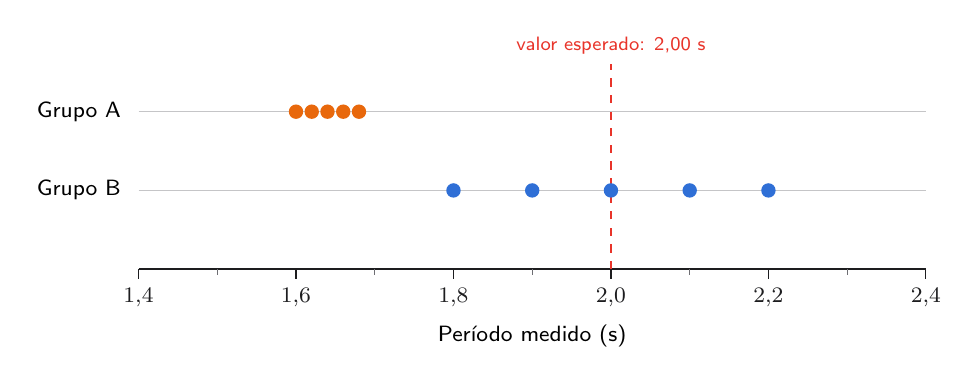
\begin{tikzpicture}[font=\footnotesize,x=10cm]
\draw[thick,tinta] (1.4,0) -- (2.4,0);
\foreach \v/\t in {1.4/1{,}4,1.6/1{,}6,1.8/1{,}8,2.0/2{,}0,2.2/2{,}2,2.4/2{,}4} {\draw[tinta] (\v,0) -- (\v,-0.12) node[below] {$\t$};}
\foreach \v in {1.5,1.7,1.9,2.1,2.3} \draw[gris] (\v,0) -- (\v,-0.07);
\node at (1.9,-0.85) {Período medido (s)};
\draw[dashed,coral,thick] (2.0,0) -- (2.0,2.6) node[above,text=coral,font=\scriptsize] {valor esperado: 2,00 s};
\node[anchor=east] at (1.39,2.0) {Grupo A};
\node[anchor=east] at (1.39,1.0) {Grupo B};
\draw[gris!40] (1.4,2.0) -- (2.4,2.0); \draw[gris!40] (1.4,1.0) -- (2.4,1.0);
\foreach \v in {1.60,1.62,1.64,1.66,1.68} \fill[nar] (\v,2.0) circle (2.6pt);
\foreach \v in {1.80,1.90,2.00,2.10,2.20} \fill[azul] (\v,1.0) circle (2.6pt);
\end{tikzpicture}
\end{document}
